\documentclass[spanish]{beamer}

%Language symbols
\usepackage[spanish]{babel}
\selectlanguage{spanish}
\usepackage[utf8]{inputenc}
\usepackage{verbatim}
\usepackage{graphicx}% http://ctan.org/pkg/graphicx
\usepackage{caption,subcaption}

% Code

\usepackage{listings,textcomp}
\lstset{literate=   % listings config
  {á}{{\'a}}1 {é}{{\'e}}1 {í}{{\'i}}1 {ó}{{\'o}}1 {ú}{{\'u}}1
  {Á}{{\'A}}1 {É}{{\'E}}1 {Í}{{\'I}}1 {Ó}{{\'O}}1 {Ú}{{\'U}}1
  {à}{{\`a}}1 {è}{{\`e}}1 {ì}{{\`i}}1 {ò}{{\`o}}1 {ù}{{\`u}}1
  {À}{{\`A}}1 {È}{{\'E}}1 {Ì}{{\`I}}1 {Ò}{{\`O}}1 {Ù}{{\`U}}1
  {ä}{{\"a}}1 {ë}{{\"e}}1 {ï}{{\"i}}1 {ö}{{\"o}}1 {ü}{{\"u}}1
  {Ä}{{\"A}}1 {Ë}{{\"E}}1 {Ï}{{\"I}}1 {Ö}{{\"O}}1 {Ü}{{\"U}}1
  {â}{{\^a}}1 {ê}{{\^e}}1 {î}{{\^i}}1 {ô}{{\^o}}1 {û}{{\^u}}1
  {Â}{{\^A}}1 {Ê}{{\^E}}1 {Î}{{\^I}}1 {Ô}{{\^O}}1 {Û}{{\^U}}1
  {œ}{{\oe}}1 {Œ}{{\OE}}1 {æ}{{\ae}}1 {Æ}{{\AE}}1 {ß}{{\ss}}1
  {ű}{{\H{u}}}1 {Ű}{{\H{U}}}1 {ő}{{\H{o}}}1 {Ő}{{\H{O}}}1
  {ç}{{\c c}}1 {Ç}{{\c C}}1 {ø}{{\o}}1 {å}{{\r a}}1 {Å}{{\r A}}1
  {€}{{\EUR}}1 {£}{{\pounds}}1 {ñ}{{\~{n}}}1
}

\lstset{    %listings config
	language=C++,
	belowcaptionskip=1\baselineskip,
	breaklines=true,
	frame=L,
	xleftmargin=0.1in,
	%otherkeywords={},
	showstringspaces=false,
	backgroundcolor=\color{white},
	basicstyle=\footnotesize\ttfamily,
	keywordstyle=\bfseries\color{purple!90!black},
	commentstyle=\itshape\color{gray!85!},
	identifierstyle=\color{blue!80!black},
	stringstyle=\color{green!60!black},
}

%Theme
\usetheme{Madrid}

%Title
\title{Práctica 4: Backtraking y Branch \& Bound}
\date{\today}
\author{José Antonio Álvarez Ocete - Norberto Fernández de la Higuera \\ Javier Gálvez Obispo - Yábir García Benchakhtir }
\institute{Doble Grado en Ingeniería Informática y Matemáticas}

%Document
\begin{document}

\frame{\titlepage}

\begin{frame}[fragile]\frametitle{Descripción del problema: el Viajante de Comercio}
\begin{figure}[H]
	\centering
	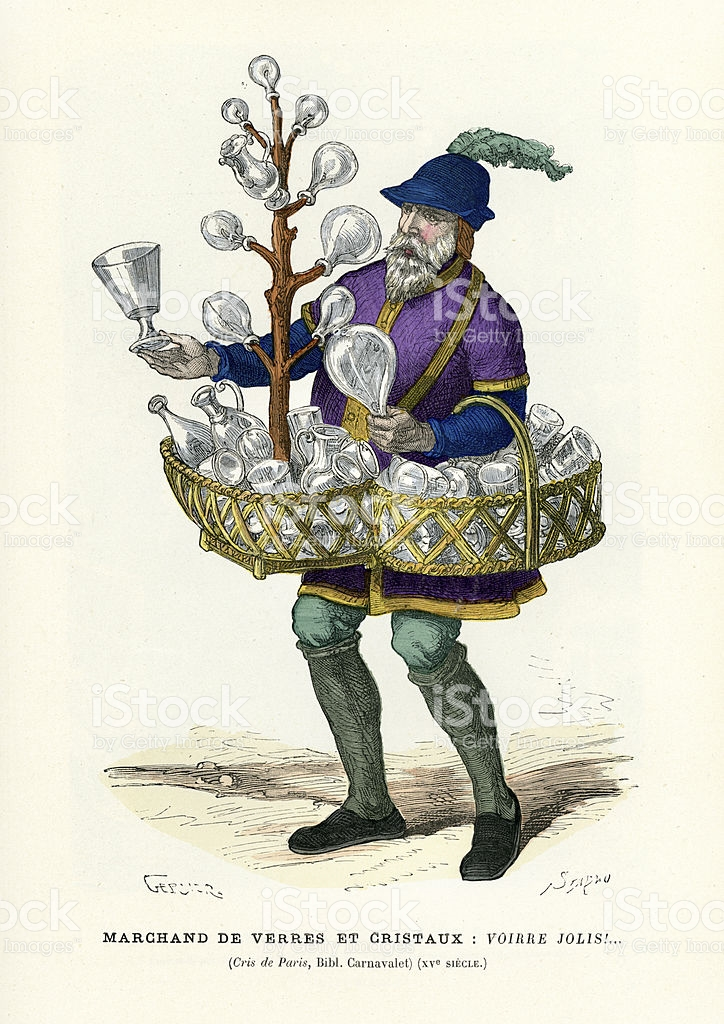
\includegraphics[width=0.47\textwidth]{comerciante.jpg}
	\caption{}
\end{figure}
\end{frame}

\begin{frame}[fragile]\frametitle{Solución branch and bound - I}

	
\end{frame}

\begin{frame}[fragile]\frametitle{Solución branch and bound - II}
	
Función de estimación utilizada:
	
\begin{lstlisting}
double estimacion(vector<int> &candidates, vector<vector<double> > &cities){
	double result = 0;
	double row_min;
	
	for(int i = 0; i < cities.size()-1; i++){
		if(!visitado(i,candidates)){
			result += rowMin(i, cities[i]);
		}
	}
	return result;
}
\end{lstlisting}
	
\end{frame}

\begin{frame}[fragile]\frametitle{Solución inicial}
	
Para decidir la ciudad de inicio para el recorrido empleamos la siguiente función:

\begin{lstlisting}[basicstyle=\tiny,]
int farthest(vector<pair<double, double> > &coordinates){
	pair<double,double> centro(0,0);
	double dist, max = 0;
	int mejor = 0;
	
	for(int i = 0; i < coordinates.size(); i++){
		centro.first += coordinates[i].first;
		centro.second += coordinates[i].second;
	}
	
	centro.first /= coordinates.size();
	centro.second /= coordinates.size();
	
	for(int i = 0; i < coordinates.size(); i++){
		dist = distance(coordinates[i], centro);
		if(dist > max){
			max = dist;
			mejor = i;
		}
	}
	
	return mejor;
}
\end{lstlisting}
\end{frame}

\begin{frame}[fragile]\frametitle{Backtracking}
Solución de backtraking implementada:
\begin{lstlisting}
void backtracking(int pos, pair<double, vector<int> > sol, vector<vector<double> > &cities, pair<double, vector<int> > &best){
	if(pos < cities.size()){
		for(int i = 1; i < cities.size(); i++){
			if(!visitado(i, sol.second)){
				sol.second[pos] = i;
				sol.first = compute_length(sol.second, cities);
				if(sol.first < best.first)
					backtracking(pos + 1, sol, cities, best);
			}
		}
	} else if(best.first < best.first)
		best = sol;
}

\end{lstlisting}
\end{frame}

\begin{frame}[fragile]\frametitle{Análisis empírico de los algoritmos}

Para estudiar la eficiencia empírica de los resultados se ha utilizado
un ordenador con las siguiente caracterísiticas:

\begin{itemize}
	\item CPU: Intel Pentium G3258 (2) @ 3.200GHz
	\item Memoria RAM: 7876MiB
	\item Kernel: 4.13.0-36-generic
	\item OS: Linux Mint 18.3 Sylvia x86\_64
\end{itemize}
\end{frame}

\begin{frame}[fragile]\frametitle{Datos obtenidos}	
\begin{table}[H]
	\centering
	\caption{Comparativa de longitud y tiempo (seg) para cada algoritmo}
	\label{my-label}
	\begin{tabular}{lll}
		\hline
		\multicolumn{1}{|l|}{Longitud} & \multicolumn{1}{l|}{Branch and bound} & \multicolumn{1}{l|}{Backtracking} \\ \hline
		\multicolumn{1}{|l|}{19.9247}  & \multicolumn{1}{l|}{3E-06}            & \multicolumn{1}{l|}{2E-06}        \\ \hline
		\multicolumn{1}{|l|}{51.6735}  & \multicolumn{1}{l|}{6E-06}            & \multicolumn{1}{l|}{3E-06}        \\ \hline
		\multicolumn{1}{|l|}{59.4593}  & \multicolumn{1}{l|}{1.7E-05}          & \multicolumn{1}{l|}{5E-06}        \\ \hline
		\multicolumn{1}{|l|}{56.4986}  & \multicolumn{1}{l|}{5E-05}            & \multicolumn{1}{l|}{1.6E-05}      \\ \hline
		\multicolumn{1}{|l|}{119.193}  & \multicolumn{1}{l|}{0.000148}         & \multicolumn{1}{l|}{6.2E-05}      \\ \hline
		\multicolumn{1}{|l|}{150.371}  & \multicolumn{1}{l|}{0.000919}         & \multicolumn{1}{l|}{0.000281}     \\ \hline
		\multicolumn{1}{|l|}{255.254}  & \multicolumn{1}{l|}{0.001052}         & \multicolumn{1}{l|}{0.000763}     \\ \hline
		\multicolumn{1}{|l|}{361.223}  & \multicolumn{1}{l|}{0.003113}         & \multicolumn{1}{l|}{0.003867}     \\ \hline
		\multicolumn{1}{|l|}{464.618}  & \multicolumn{1}{l|}{0.015933}         & \multicolumn{1}{l|}{0.021076}     \\ \hline
		\multicolumn{1}{|l|}{476.531}  & \multicolumn{1}{l|}{0.014079}         & \multicolumn{1}{l|}{0.049719}     \\ \hline
		\multicolumn{1}{|l|}{586.246}  & \multicolumn{1}{l|}{0.193942}         & \multicolumn{1}{l|}{3.49537}      \\ \hline
		\multicolumn{1}{|l|}{755.058}  & \multicolumn{1}{l|}{0.046548}         & \multicolumn{1}{l|}{0.676337}     \\ \hline
		\multicolumn{1}{|l|}{1040.99}  & \multicolumn{1}{l|}{0.234971}         & \multicolumn{1}{l|}{9.97742}      \\ \hline
		&                                       &                                  
	\end{tabular}
\end{table}
\end{frame}

\begin{frame}[fragile]\frametitle{Comparativa gráfica}	
\begin{figure}[H]
	\centering
	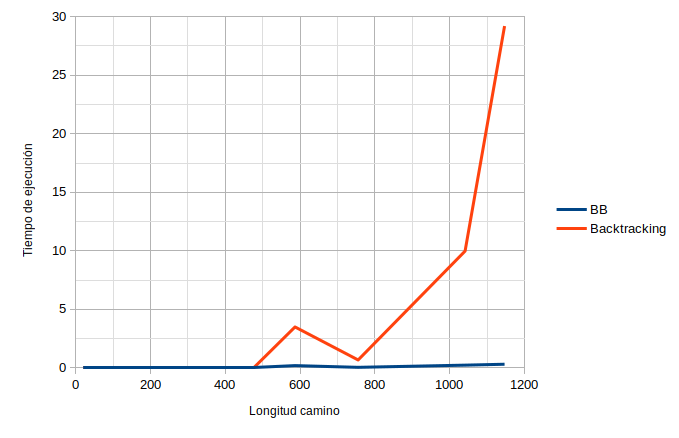
\includegraphics[width=0.8\textwidth]{comparativa.png}
	\caption{Comparativa de los algoritmos de backtracking y branch and bound}
\end{figure}
\end{frame}

\begin{frame}[fragile]\frametitle{Comparativa con los algoritmos greedy}
\begin{table}[H]
	\centering
	\caption{Resultados para un algoritmo greedy}
	\label{my-label}
	\begin{tabular}{|l|l|}
		\hline
		19.9247 & 4E-06 \\ \hline
		51.6735 & 2E-06 \\ \hline
		59.4593 & 1E-06 \\ \hline
		62.8659 & 2E-06 \\ \hline
		123.26  & 2E-06 \\ \hline
		150.371 & 3E-06 \\ \hline
		300.216 & 3E-06 \\ \hline
		361.223 & 3E-06 \\ \hline
		494.908 & 2E-06 \\ \hline
		476.531 & 4E-06 \\ \hline
		794.865 & 4E-06 \\ \hline
		581.918 & 4E-06 \\ \hline
		1005.65 & 5E-06 \\ \hline
		1070.15 & 5E-06 \\ \hline
	\end{tabular}
\end{table}
\end{frame}

\begin{frame}[fragile]\frametitle{Comparativa de caminos - I}
\begin{figure}[H]
	\centering
	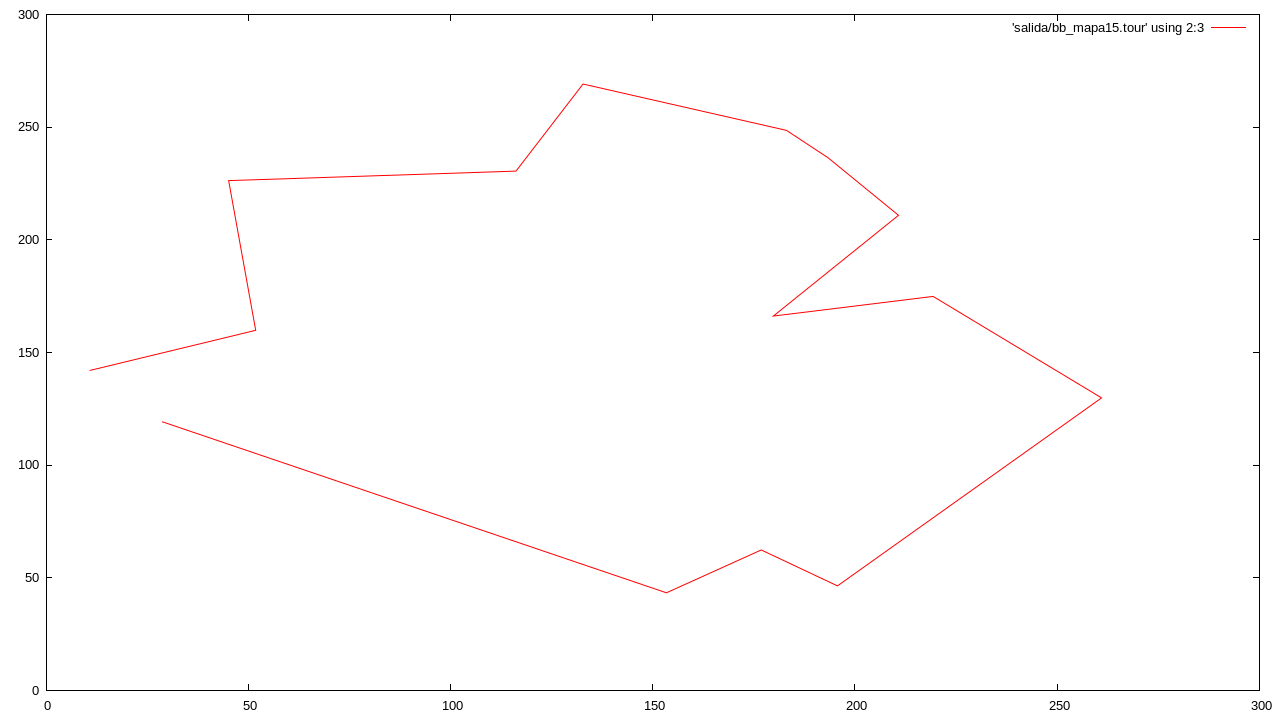
\includegraphics[width=0.8\textwidth]{bb_mapa15}
	\caption{Algoritmo de branch and bound}
\end{figure}
\end{frame}

\begin{frame}[fragile]\frametitle{Comparativa de caminos - II}
\begin{figure}[H]
	\centering
	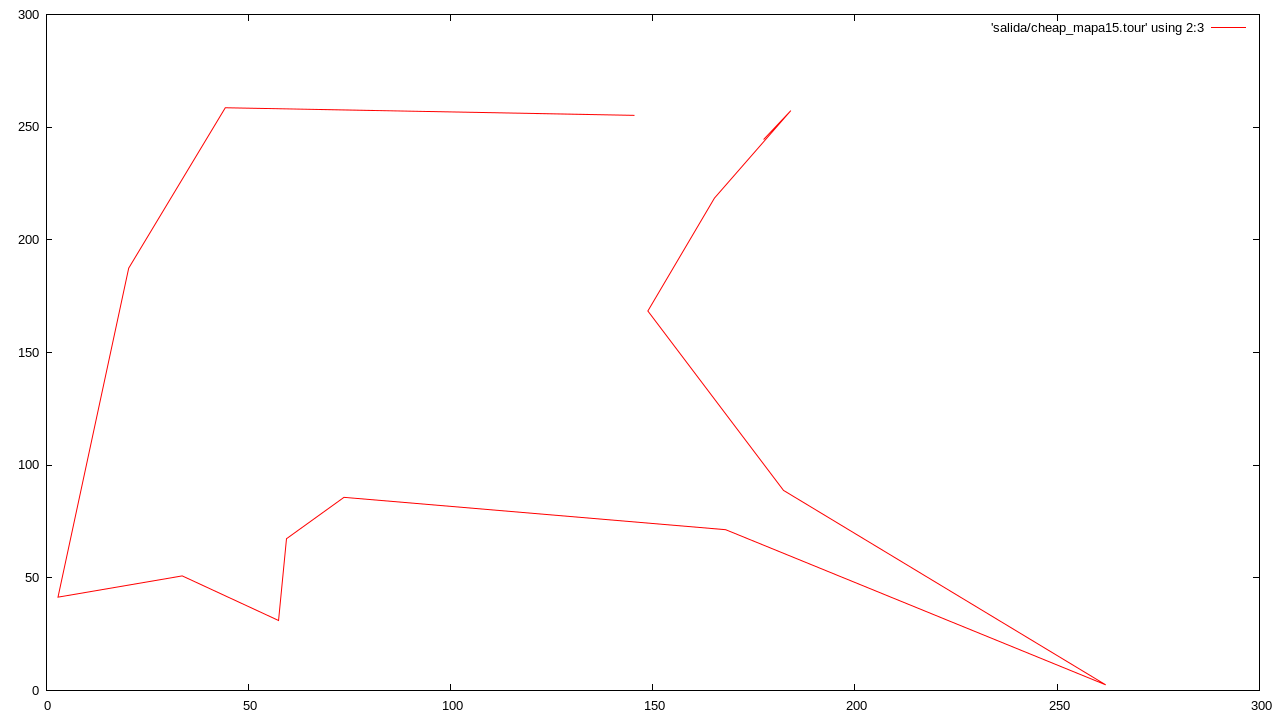
\includegraphics[width=0.8\textwidth]{cheap_mapa15}
	\caption{Algoritmo greedy}
\end{figure}
\end{frame}

\begin{frame}\frametitle{Conclusiones}
	\begin{figure}[H]
		\centering
		
\includegraphics[width=0.6\textwidth]{mario}
	\end{figure}
\end{frame}

\end{document}